\begin{df} 
    Przestrzeń topologiczna $(X,\mathcal{T})$, gdzie $\mathcal{T}$ jest rodziną podzbiorów $X$
    taką, że $\emptyset,X \in \mathcal{T}, \ \mathcal{T}$ jest zamknięta na skończone przekroje oraz 
    dowolne sumy. \\
    $\mathcal{T}$ - topologia, $U \in \mathcal {T}$, to $U$ jest zbiorem otwartym.
\end{df} 
\section{Topologia naturalna na $\mathbb{R}$ }
\begin{df}
    $ U \subseteq \mathbb{R}$ jest otwarty, jeżeli dla każdego $x$ istnieje $\delta > 0$, taka, że $(x - \delta, x+\delta) \subseteq U$. \\
    $ \forall x \in U \ \exists \, \delta > 0 \ (x-\delta,x+\delta) \subseteq U $.
\end{df}
\begin{minipage}[c]{0.5\linewidth}
\begin{przy} \hfill 
    \begin{itemize} 
        \item $\emptyset$ jest otwarty i domknięty.
        \item $\mathbb{R}$ jest otwarty i domknięty.
        \item $(a,b)$ jest otwarty, np. $\delta = \frac{\min(x-a,b-x)}{2}$
    \end{itemize} 
\end{przy} 
\end{minipage}
\begin{minipage}[b]{0.4\linewidth}
    \begin{tikzpicture}
        \draw (0,0) -- (5,0);
        \draw[fill] circle[radius=0.025] node[below]{$a$};
        \draw[fill] (5,0) circle[radius=0.025] node[below]{$b$};
        \draw[fill] (0.4,0) circle[radius=0.025] node[above]{$x$};
    \end{tikzpicture}
\end{minipage} 
\begin{df} 
    $ F \subseteq \mathbb{R} $ jest domknięty jeżeli: $\mathbb{R} \setminus F$ jest otwarty. 
    $ \forall x \notin F \ \exists \, \delta > 0 \ ( x - \delta, x + \delta ) \cap F = \emptyset $.
\end{df} 
\begin{przy} \hfill
    \begin{itemize} 
        \item $(0,1)$ nie jest domknięty, $0 \notin (0,1)$, ale dla $\delta > 0, \ (-\delta,\delta) 
                \cap (0,1) \neq \emptyset$
        \item $[0,1]$ jest domknięty.
        \item $[0,1)$ nie jest otwarty i nie jest domknięty.
    \end{itemize} 
\end{przy}
\begin{tw} 
    \hfill
    \begin{enumerate}[{(}1{)}]
        \item Jeżeli $U$ i $V$ są otwarte to $U \cap V $ jest otwarty. 
        \item Jeżeli $\{U_t : t \in T\}$ jest rodziną otwartą, to $ \bigcup\limits_{t \in T} U_t $ jest otwarty.
    \end{enumerate}
\end{tw} 
\begin{dd} 
    ~\newline
    Niech $x \in U \cap V$. Wtedy 
    \begin{tabular}[t]{l} 
    $x \in U $, U otwarty, więc istnieje $\delta_1 \ (x-\delta_1,x+\delta_1) \subseteq U$.\\
    $x \in V$, V otwarty, więc istnieje $\delta_2 \ (x-\delta_2,x+\delta_2) \subseteq V.$ \\ 
    Zatem dla $\delta = \min(\delta_1,\delta_2), \ (x-\delta,x+\delta) \subseteq U \cap V$.
    \end{tabular} \\[5mm]
    Niech $x \in \bigcup\limits_{t \in T} $. Wtedy istenieje $t_0 \in T$,
    takie, że $x \in U_{t_0}$. $U_{t_0}$ otwarty, więc istnieje $\delta > 0$,
    takie, że $( x - \delta, x+\delta) \subseteq U_{t_0} \subseteq \bigcup\limits_{t \in T} U_t $
    \qed
\end{dd}
\begin{uw}
    Przekrój ciągu zbiorów otwartych nie musi być otwarty.
\end{uw}
\begin{prz}
    Przekrój ciągu zbiorów otwartych nie musi być otwarty
    \[ [0,1] = \bigcap_{n=1}^\infty (-\frac{1}{n},1+\frac{1}{n}) \]
\end{prz}
\begin{uw} 
    \hfill
    \begin{enumerate}[(1)]
        \item Jeżeli $F$ i $H$ są domknięte to $F \cup H$ jest domknięty. 
        \item Jeżeli $\{ F_t : t \in T \}$ jest rodziną zbiorów domkniętych to $\bigcap\limits_{t \in T} F_t$ jest domknięty.
    \end{enumerate}
\end{uw}

\begin{tw}
    dla $f: \mathbb{R} \rightarrow \mathbb{R}$, NWSR: 
    \begin{enumerate}[(i)]
        \item f jest ciągła 
        \item dla dowolnego otwartego $V \subseteq \mathbb{R}, \  f^{-1}[V]$ jest otwarty.  
        \item dla dowolnego domkniętego $ F \subseteq \mathbb{R}, \ f^{-1}[F]$ jest domknięty. 
    \end{enumerate}
\end{tw}

\begin{dd} 
    \hfill
    \begin{itemize} 
        \item[(i) $\Rightarrow $ (ii)] Niech $V \subseteq \mathbb{R}$ będzie otwarty. Niech $ x \in f^{-1}[V]$.
            Zatem $f(x) \in V. \ V$ jest otwarty, wiec istnieje 
            $\varepsilon > 0 \\ (f(x)-\varepsilon,f(x)+\varepsilon) \subseteq V$.
            Z ciągłości, w sensie Cauchy'ego, istnieje $\delta > 0$, taka, że $|x - y| < \delta 
            \Rightarrow |f(x) - f(y)| < \varepsilon$. 
            Jeżeli $|y - x| < \delta$, to $f(y) \in V \Rightarrow (x-\delta,x+\delta) \subseteq f^{-1}[V]$ 
        \item[(ii) $\Rightarrow$ (iii)] Niech $F$ będzie domknięty. 
        $\mathbb{R} \setminus f^{-1}[F] = f^{-1}[\underscript{\mathbb{R}\setminus F}{\uparrow}{\text{otwarty}}].$
    \end{itemize} 
    Dowody dla (iii) $\Rightarrow$ (ii) oraz (ii) $\Rightarrow$ (i) są analogiczne. \hfill \qed
\end{dd} 

\begin{tw}
    Dla zbioru $U \subseteq \mathbb{R}$, NWSR:
    \begin{enumerate}[(i)]
        \item $U$ jest otwarty 
        \item $U = \bigcup\limits_{t \in T} (a_t,b_t)$ dla pewnych $a_t,b_t \in \mathbb{R}$
        \item $U = \bigcup\limits_{n=1}^\infty (c_n,d_n)$ dla pewnych $c_n,d_n \in \mathbb{R}$
    \end{enumerate}
\end{tw}

\begin{dd}
    (iii) $\Rightarrow$ (ii) $\Rightarrow$ (i) oczywiste 
    \begin{itemize} 
        \item[(i) $\Rightarrow$ (ii)] Dany jest zbiór otwarty $U \subseteq \mathbb{R}$. 
            Dla $x \in U \ \exists \, \delta_x > 0 \ 
            (\underbrace{x-\delta_x}_{a_x},\underbrace{x+\delta_x}_{b_x}) \subseteq U$, 
            czyli $U = \bigcup\limits_{x \in U} (a_x,b_x)$.
        \item[(ii) $\Rightarrow$ (iii)] Rodzina $\{(p,q) : p,q \in \mathbb{Q}\}$ jest przeliczalna. 
            $U = \bigcup\limits_{x \in U} (p_x,q_x) = \bigcup\limits_{n=1}^\infty (c_n,d_n)$    
            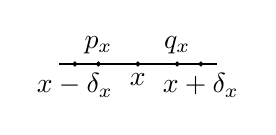
\begin{tikzpicture}
                \draw (0,0) -- (2,0);
                \draw[fill] (1,0) circle[radius=0.025] node[below]{$x$};
                \draw[fill] (0.2,0) circle[radius=0.025] node[below]{$x-\delta_x$};
                \draw[fill] (1.8,0) circle[radius=0.025] node[below]{$x+\delta_x$};
                \draw[fill] (0.5,0) circle[radius=0.025] node[above]{$p_x$};
                \draw[fill] (1.5,0) circle[radius=0.025] node[above]{$q_x$};
            \end{tikzpicture}
    \end{itemize} \hfill \qed
\end{dd}

\begin{lem}
    Niech $[a,b] \subseteq \bigcup\limits_{n=1}^\infty (a_n,b_n)$, wtedy istnieje $N \in \mathbb{N}$, t. że $\bigcup\limits_{n=1}^N (a_n,b_n) \supseteq [a,b]$.
    \begin{dd}
        $S = \{ x: a \le x \le b$, przedział $[a,x]$ przykrywa się skończoną ilością $(a_n,b_n)\}$ \\
        $S \neq \emptyset$, bo $a \in S$. $S$ jest ograniczony z góry. Niech $s = \sup S$. \\
        $ s \in [a,b] \subseteq \bigcup\limits_{n=1}^\infty (a_n,b_n)$. \\
        Istnieje $n_0, s \in (a_{n_0},b_{n_0})$. Istnieje $x \in S \ a_{n_0} < x < s $. \\
        Istnieje $N \ [a,x] \subseteq \bigcup\limits_{n=1}^N (a_n,b_n).$ \\
        $[a,s] \subseteq \bigcup\limits_{n=1}^{N'} \quad N' = \max(N,n_0)$ \\
        Zostało pokazać, że $s = b$. Można to zrobić w podobny sposób.
    \end{dd}
\end{lem}

\begin{wn}
    Dla $a \le b$ przedział $[a,b]$ jest zwarty, to znaczy z każdego pokrycia $[a,b]$ zbiorami otwartymi, 
    można wybrać pokrycie skończone.
\end{wn}

\begin{wn}
    Jeżeli $f: \mathbb{R} \rightarrow \mathbb{R}$ jest ciągła, to $f$ jest ograniczona na $[a,b]$.
\end{wn}
\begin{dd} 
    $[a,b] \subseteq f^{-1}[\mathbb{R}]  = \bigcup\limits_{n=1}^\infty f^{-1}[(-n,n)]$. 
    Z zwartości istnieje $n_0$, takie, że $[a,b] \subseteq f^{-1}[(-n_0,n_0)]$.
\end{dd} 

\begin{tw} 
    Każdy ciąg $x_n \in [0,1]$ ma podciąg zbieżny. 
\end{tw} 
\begin{dd} 
    Pokażemy, że istnieje $a \in [0,1]$, takie, że dla dowolnego 
    $\delta > 0, \ x_n \in (a-\delta,a+\delta)$ dla nieskończone wielu n. \\
    Wtedy dla $\forall k \in \mathbb{N} \ \exists n_k > n_{k-1} \quad x_{n_k} \in (a-\frac{1}{k},a+\frac{1}{k}).$ \\ 
    Załóżmy nie wprost, że $\forall a \in [0,1] \ \exists \delta_a > 0 \ (a-\delta_a,a+\delta_a)$ 
    zawiera skończenie wiele wiele wyrazów ciągu. \\
    $[0,1] \subseteq \bigcup\limits_{a \in [0,1]} (a-\delta_a,a+\delta_a) $. 
    Ze zwartości $[0,1] \subseteq \bigcup\limits_{n=1}^K (a_i-\delta_{a_i},a_i+\delta_{a_i}) $. \lightning \\ 
    (po lewej zawiera wszystkie wyrazy ciągu, po prawej tylko skończenie wiele)
\end{dd}

\begin{tw} 
    $\mathbb{R}$ jest spójna, to znaczy nie istnieje podział prostej na dwa zbiory otwarte rozłączone.
\end{tw} 
\begin{dd}
    Niech $U,V \neq \emptyset,$ otwarte, $ U \cap V = \emptyset, \ U \cup V = \mathbb{R}$.
    Niech $a \in U, \ b \in V, s = \sup (U \cap [a,b])$. \\ Skoro $s \in U$, to istnieje $\delta > 0$, 
    taka, że $(s-\delta,s+\delta) \subseteq U$, sprzeczność z definicją supremum.
\end{dd}

